% !TEX root = ../my-thesis.tex
%
\chapter{EXPERIMENTACIÓN Y RESULTADOS}
\label{sec:resultados}

A lo largo de este capítulo, se mostrarán y explicarán los diferentes experimentos que han sido necesarios realizar durante la elaboración de este trabajo. También se realizará una discusión sobre los resultados, comprobando si las hipótesis inicialmente formuladas son verificadas.

\section{Entorno de ejecución}
El entorno de ejecución y trabajo empleados para el desarrollo de las pruebas realizadas es un punto totalmente vital para la correcta elaboración de este trabajo. Esto es debido a la naturaleza del propio trabajo, el cuál tiene como objetivo el resolver un problema con un requerimiento computacional muy alto.

El entrenamiento de Redes Neuronales es un problema de optimización intrínsecamente paralelo. Es por esto que es de gran importancia el contar con un hardware de trabajo adecuado.

En los últimos años, se ha comprobado como las \textbf{GPUs} (\textit{Graphics Processing Units}) han sido clave para la rápida escalada de estos algoritmos en el uso y resolución normal de problemas. Esto es debido a lo que anteriormente se comentaba, y es que la arquitectura intrínseca de las mismas permiten un gran avance en el procesamiento y el cálculo en paralelo, justo al contrario de lo que sucede con las habituales \textbf{CPUs} (\textit{Central Processing Units}).

Debido a todo esto, un punto totalmente vital de este trabajo es la capacidad computacional de la que se tiene disponible para la realización de esta experimentación, ya que se necesitan de máquinas preparadas específicamente para este tipo de propósitos. Esta nos debe dar facilidades y herramientas para la ejecución de programas de gran tiempo de ejecución y con diferentes configuraciones.

Por todo lo anterior comentado resulta imposible la ejecución de estos programas en un ordenador tradicional, por lo que se requerirá la búsqueda y prueba de grandes infraestructuras de computación preparados para el desarrollo de este tipo de tecnologías. Estas disponen de hardware especializado para estos desarrollos y se ponen a disponibilidad de la comunidad investigadora para su uso.

Debido a que estas son compartidas, contarán con diferentes limitaciones para no monopolizar el uso de las mismas, por lo que se tendrán limitaciones temporales de ejecución, de horas totales, de prioridad y de solicitud de hardware disponible. Es por ello que el conocimiento de estas limitaciones y la adaptación a ellas son totalmente necesarias para la adecuada ejecución de los programas.

Los largos tiempos de ejecución necesarios para el lanzamiento de diferentes topologías de redes convolucionales y su entrenamiento lleva a ingeniarse diferentes soluciones para disminuir el tiempo de cómputo de forma eficiente, como se verán en próximos capítulos.

\subsection{Artemisa}
\textbf{Artemisa} (\textit{ARTificial Environment for ML and Innovation in Scientific Advanced Computing}) \footnote{\url{https://artemisa.ific.uv.es/web/}} es la infraestructura de computación dedicada a inteligencia artificial desarrollada por el \textbf{IFIC} (\textit{Instituto de Física Corpuscular}) asociado al \textbf{CSIC} y a la \textit{Universitat de València}.

Esta plataforma de computación esta dedicada a técnicas de Inteligencia Artificial como \textit{Machine Learning} y \textit{Big Data}. Esta se desarrolla a partir del centro de cálculo del IFIC, la cual dentro del \textit{Programa operativo FEDER de la Comunitat Valenciana 2014-2020} aportó la financiación necesaria para la adquisición de la infraestructura y equipamiento. Este alberga dentro de uno de sus nodos dedicados a la red de computación (\textit{Grid}) los datos obtenidos por el experimento ATLAS del LHC entre otros experimentos. 

En la figura \ref{fig:artemisa}, se puede ver una fotografía de como es físicamente una parte de esta plataforma de computación.

\begin{figure}[ht]
    \centering
    \includegraphics[width=1.0\textwidth]{figuras/centro_calculo_ific.jpg}
    \caption{Fotografía de la plataforma de computación Artemisa}
    \label{fig:artemisa}
\end{figure}

Artemisa dispone de un sistema de cálculo de altas prestaciones multi-GPU para el desarrollo de aplicaciones basadas en Inteligencia Artificial. Cuenta actualmente con 23 servidores que alojan varias tarjetas gráficas especialmente desarrolladas para el cálculo en Inteligencia Artificial, que van a ser usados en modo \textit{batch} y donde podemos encontrar varias interfaces. Además de esto, Artemisa cuenta con CPUs de última generación y con sistemas de almacenamiento de gran velocidad.

Artemisa se desarrolla bajo el sistema operativo de \textit{Linux Centos 7}, que se trata de una distribución libre basada en \textit{Red Hat Enterprise Linux (RHEL) 7}. Además trae instalado numerosas herramientas que son de utilidad para el lanzamiento y ejecución de programas. En el caso de este trabajo, destacar \textit{Python 3.6.1}, el uso de los \textit{Containers} de \textit{Dockers} y los \textit{Virtual Environment} de \textit{Python}.

\subsection{Hardware}
Dada a la importancia del hardware de este para la ejecución de nuestros programas presentaremos cuales están instalados en Artemisa ya que a más potente o mejor preparado este para nuestro problema, más rápidamente y eficientemente se realizarán las ejecuciones.

El hardware de Artemisa se estructura en nodos de tres clases diferentes:
\begin{itemize}
    \item \textbf{Interfaces de Usuario (UI):} es el punto de entrada del usuario, facilitando un entorno de trabajo donde compilar y probar sus programas. Cuando un \textit{job} esta disponible, los usuarios pueden subir desde aquí los diferentes paquetes de trabajo con el \textit{Job Management System} a los \textit{Nodos de Trabajo}
    \item \textbf{Nodos de Trabajo (WN):} donde los usuarios pueden ejecutar sus paquetes de trabajo. Contiene CPUs de gran potencia, gran cantidad de memoria y 4 \textit{GPGPU} de gran velocidad.
    \item \textbf{Nodos de Almacenamiento:} son servidores donde el usuario puede almacenar sus datos y los datos de sus proyectos, y son accesibles tanto por las \textit{Interfaces de Usuario} como por los \textit{Nodos de Trabajo}.
\end{itemize}

A continuación se presenta el hardware del que está compuesto Artemisa:

\begin{itemize}
    \item 2 Interfaces de Usuario (mlui01.ific.uv.es, mlui02.ific.uv.es) con:
    \begin{itemize}
        \item 2 x Intel Xeon Gold 6130 CPU @ 2.10GHz 16c
        \item 192 GBytes ECC DDR4 a 2666 MHz
        \item 1 x GPU Tesla Pascal P100 PCIe
    \end{itemize}
    \item 2 x Nodos de Trabajo con:
    \begin{itemize}
        \item 2 x Intel Xeon Platinum 8160 CPU @ 2.10GHz 24c
        \item 384 GBytes ECC DDR4 a 2666 MHz
        \item 1 x GPU Tesla Volta V100 PCIe
    \end{itemize}
    \item 20 x Nodos de Trabajo con:
    \begin{itemize}
        \item 2 x Intel(R) Xeon(R) Gold 6248 CPU @ 2.50GHz 20c
        \item 384 GBytes ECC DDR4 a 2933 MHz
        \item 1 x GPU Tesla Volta V100 PCIe
    \end{itemize}
    \item 1 x Nodos de Trabajo con:
    \begin{itemize}
        \item 2 x Intel Xeon Platinum 8180 CPU @ 2.50GHz 28c
        \item 768 GBytes ECC DDR4 s 2666 MHz
        \item 4 x GPU Tesla Volta V100 SMX2
    \end{itemize}
    \item 5 x Servidores de Almacenamiento con:
    \begin{itemize}
        \item 2 x Intel Xeon Gold 6130 CPU @ 2.10GH 16c
        \item 192 GBytes ECC DDR4 a 2666 MHz
        \item 6 x 8TB SAS 12 Ggb/s SEAGATE ST8000NM0065
    \end{itemize}
\end{itemize}

Además de esto, su conexión es de vital importancia, ya que a estos dispositivos el acceso se hace de forma totalmente remota, es por ello que se cuenta con conexión \textbf{Ethernet de 10 Gbps} dentro de toda la instalación.

\subsection{HTCondor}
Artemisa necesita una administración eficiente del hardware disponible (\textit{Job Management System}), ya que sino de otra forma se estaría desperdiciando todo su potencial. Es por ello que este integra el software de \textbf{HTCondor} \footnote{\url{https://research.cs.wisc.edu/htcondor/}}. Este permite la creación de un entorno de computación de alto rendimiento (HTC). Además ayuda a extraer eficazmente la potencia informática de las diferentes máquinas conectadas en la red. Esto viene dado debido al desarrollo en el provecho de recursos compartidos con la propiedad distribuida.

Para trabajar con este, como usuario, se ha de enviar los diferentes trabajos a HTCondor. Este es capaz de localizar las máquinas disponibles y ejecuta los trabajos allí. Además, en caso de fallo de una de las máquinas, HTCondor gestionará su ejecución en otra que este disponible de forma automatizada.

Por parte del usuario, facilita en gran medida ejecutar diferentes instancias de un mismo programa de manera sencilla durante largo tiempo de ejecución, despreocupándose de problemáticas que puedan ir apareciendo. Aún así, permite la configuración del lanzamiento de su código, solicitando una cantidad mínima de hardware necesario para la correcta ejecución, que este software lo administrará para hacerlo de forma adecuada.

Debido a que el uso de Artemisa es compartido por varios usuarios, HTCondor es capaz de administrar el hardware y poner limitaciones a cada uno de ellos, evitando monopolizar el tiempo y la potencia de esta infraestructura. Es por ello que puede priorizar diferentes trabajos a usuarios que hayan realizado menor tiempo de ejecución en el sistema.

Artemisa cuenta con varias limitaciones para asegurar el reparto equitativo del uso de la herramienta. Es por ello, que el desarrollo del programa de ejecución debe estar en la línea de estas limitaciones, para tratar de que afecten a su ejecución lo menos posible. Algunas de estas limitaciones son:

\begin{itemize}
    \item Máximo tiempo de ejecución: 48 horas
    \item Máximos \textit{Cores} disponibles: 8
    \item Máxima memoria disponible: 32768 MB
    \item Máximas GPUs disponibles: 4
\end{itemize}

Teniendo en cuenta estas limitaciones, se ha tenido que desarrollar una serie de adaptaciones al código a partir de la generación de \textit{Checkpoints} para la ejecución de programas durante tiempos superiores a 48 horas. De esta manera se puede retomar ejecuciones de programas exactamente por el punto donde se había quedado anteriormente, lo que flexibiliza y facilita mucho la investigación acerca del área que se está tratando.


\section{Experimentos y Discusión}

En esta sección, se pasarán a verificar diferentes hipótesis que se han ido elaborando a lo largo del desarrollo del trabajo. Para esto, se presentarán diferentes experimentos que consigan abarcar esta verificación y finalmente, se desarrollarán ciertas discusiones alrededor de los resultados obtenidos.

\subsection{Experimento 1. Número de capas máximo de las CNNs}

El número de capas de las CNNs, es un parámetro vital en el proceso de generación del genotipo dentro del Algoritmo Genético y para el posterior desempeño de su fenotipo a la hora de generar la arquitectura de la CNN. Es por ello que una elección de este valor es totalmente esencial para la creación de arquitecturas de CNNs adecuadas para la resolución de clasificación de imágenes.

Se busca que las redes tengan tamaños reducidos, que sean capaces de competir con redes existentes actuales para la clasificación de imágenes. A pesar de esto, un número bajo de capas puede producir una peor resolución de este problema, ya que no son capaces de extraer la cantidad suficiente de características necesarias para clasificar las imágenes de entrada.

Por otro lado, un valor demasiado grande de capas, puede hacer que exista información dentro del genotipo que no se manifieste nunca, ampliando de manera muy amplia el espacio de búsqueda de soluciones. Además, puede llevar de la misma manera a generar redes demasiado lentas de entrenar, que nos desvíen del objetivo propuesto en este trabajo.

Es por esto, que se propone la realización de este experimento, para obtener un número de capas adecuado, donde se puedan generar una gran variedad de estructuras de CNNs suficientemente buenas para obtener un clasificador suficientemente robusto y óptimo para la problema propuesto.

Para esto, se han observado como son los individuos que se generan con un máximo de capas de 10, 12, 14, 16 y 20 en diferentes ejecuciones, viendo como es la evolución de estos a lo largo del tiempo. Posteriormente, se monitoriza cuando el número de capas máximo establecido resulta una limitación para la generación libre del número de capas que tienen los individuos generados.

\begin{table}[h]
\caption{Evolución de los individuos que no se limitan por el número de capas máximo establecidos en los parámetros}
\label{tab:numero_capas}
\centering
\begin{tabular}{l|rrrrr}
\toprule
\textbf{Número de capas máximo}            & 10   & 12   & 14   & 16   & 20   \\ \hline
\textbf{\% de individuos con menos capas} & 65,9 & 84,7 & 93,8 & 94,8 & 99,1\\
\bottomrule
\end{tabular}
\end{table}

En la Tabla \ref{tab:numero_capas}, se puede observar como es la evolución anteriormente comentada, es la esperada, disminuyendo el número de individuos limitados cuanto más grande es el número de capas máximo. Se observa un gran salto a partir del número de capas 14, pasando a ser solo cerca del 6\% de los individuos que se ven limitados. Por tanto, se cree adecuado tomar valores superiores a este, para verificar que esta limitación no perjudica en gran medida las desempeño de las redes generadas.

Aún así, un valor muy a tener en cuenta es el de 20 capas máximo, ya que se puede observar que menos del 1 \% de los individuos se ven restringidos por esta limitación, no siendo muy superiores además los tiempos totales de ejecución del algoritmo.


\subsection{Experimento 2. CNNs generadas con tamaño de entrada a \textit{Fully Connected Layers} demasiado grande}

Hay ocasiones, que debido a la naturaleza de la estructura de la CNN generada, puede que las imágenes procesadas de la última capa no hayan conseguido llegar a un tamaño suficientemente reducido para que posteriormente sea procesado por la capa \textit{Fully Connected} para su clasificación. 

Se sostiene la hipótesis que esto podría llevar a un aumento considerable de los tiempos de procesamiento y que el rendimiento de la red sea bastante menor de lo esperado, si esto sucede. Esto se pensó así, debido a la estructura que tienen las redes neuronales convolucionales más empleadas actualmente, donde como se puede ver en la Tabla \ref{tab:ultima_capa_redes}, el tamaño de las FM en esta última capa, era más o menos constante y comprendido en un rango, por lo que se pensó en considerar como individuos malos los individuos que no siguieran esta forma, descartándolos de la siguiente población.

\begin{table}[h]
\caption{Tamaño de la \textit{Feature Map} en la última capa de las redes más empleadas en la actualidad}
\label{tab:ultima_capa_redes}
\centering
\begin{tabular}{l|c}
\toprule
\textbf{Red Neuronal Convolucional} & \multicolumn{1}{l}{\textbf{Tamaño última capa}} \\ \hline
LeNet \cite{lesnet}                             & 5x5      \\
AlexNet \cite{NIPS2012_c399862d}                            & 6x6  \\
VGG-16 \cite{simonyan2015deep}                             & 7x7 \\
Inception V1 \cite{szegedy2014going}                       & 7x7 \\
Inception V3 \cite{szegedy2015rethinking}                       & 8x8   \\
Resnet-50 \cite{He2016}                          & 7x7                                             \\
Xception \cite{chollet2017xception}                           & 10x10  \\
Inveption V4 \cite{szegedy2016inceptionv4}                       & 8x8 \\
ResnetXT-50 \cite{xie2017aggregated}                        & 7x7      \\
\bottomrule
\end{tabular}
\end{table}

Es por ello, que con este experimento, se pretende investigar si es adecuado descartar estar redes y denominarlas como redes \textit{no válidas} y asignarles un valor de \textit{fitness} igual a cero para que sean descartadas, o por el contrario, intentar obtener un valor de \textit{fitness} tratando de entrenar la red y valorando el material importante que pueda llevar codificada este individuo.

Para esto, se comienza partiendo de una implementación realizada con esta limitación puesta, donde los individuos que no hayan conseguido que su última capa, antes de la \textit{FCL}, reducir el tamaño de la imagen de entrada a un tamaño de las \textit{Feature Maps} de 8x8, serán descartados. Al realizar esta prueba, se descubre como en más del 50\% de generaciones, al menos un individuo es descartado, y por tanto, se limita la propagación de partes de su genotipo que podrían llegar a ser buenas, viéndose finalmente, la existencia de poca diversidad genética dentro de la población.

\begin{figure}[h]
    \centering
    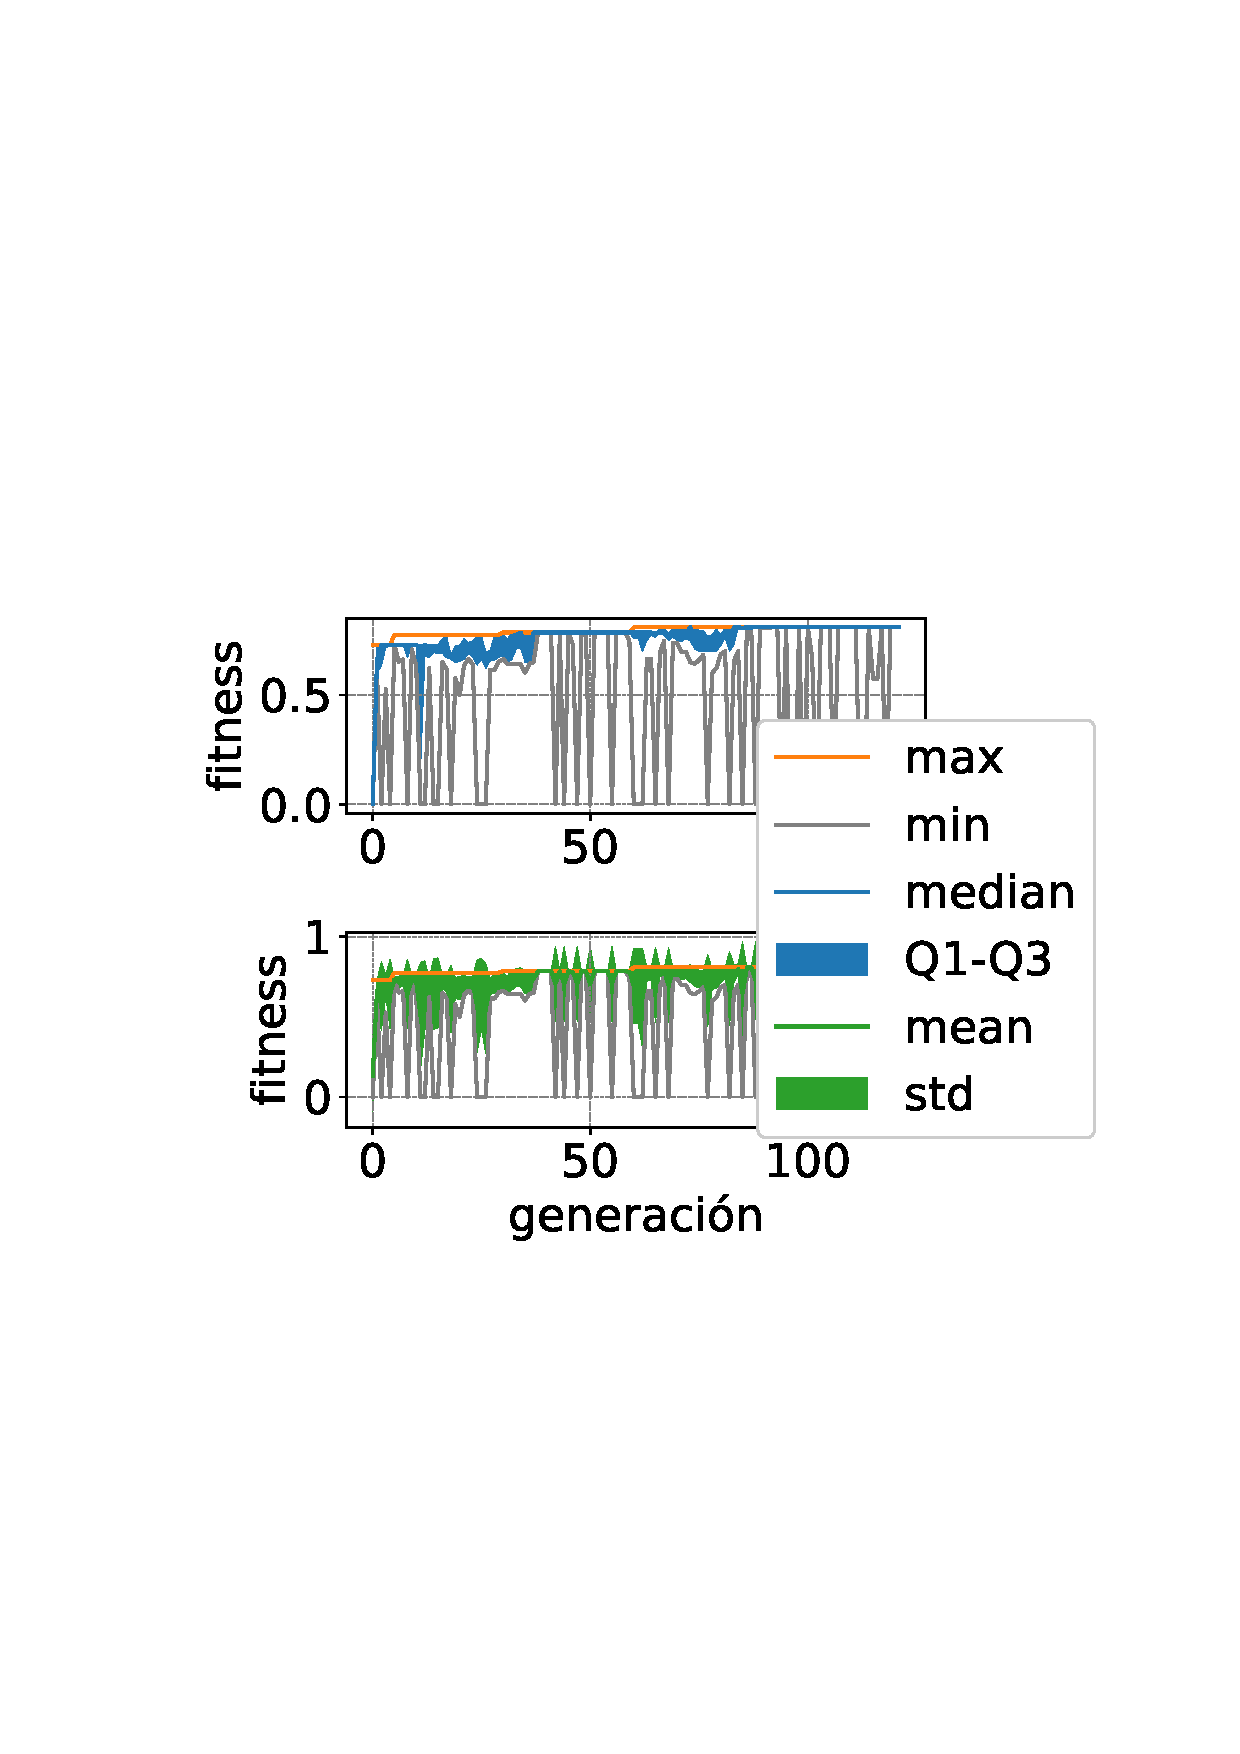
\includegraphics[width=1\textwidth]{figuras/experimentos/fcl_grande/con_limitacion_1.pdf}
    \caption{Muestra de evolución de la implementación con limitación en el tamaño de \textit{FM} a la entrada de la \textit{FCL}}
    \label{fig:con_limit_fcl}
\end{figure}

Esto que se comenta se puede ver claramente en la Figura \ref{fig:con_limit_fcl}, donde se generan gran cantidad de individuos válidos, a lo largo de las diferentes generaciones, haciendo que el algoritmo evolutivo no valore suficientes individuos de forma adecuada. Además, se ve una rápida convergencia del algoritmo a una solución no demasiado buena, con apenas un \textit{fitness} de 0,81 para el mejor individuo en ambas ejecuciones.

En total se lanzaron 8 ejecuciones, consiguiendo resultados equivalentes a las mostradas anteriormente, en todas ellas.

Tras esta apreciación, se ha de comprobar si realmente resulta una limitación real el entrenamiento de estos individuos, que no tienen una forma igual o similar a las arquitecturas encontradas en la literatura. En esto se descubre que lejos de ser una limitación para el Algoritmo Evolutivo, el algoritmo genética funciona de manera más lógica, sin descartar de forma contundente a ninguno de los individuos, y calificando a estos con una \textit{fitness} proporcional a su desempeño en la clasificación de las imágenes de entrada.

\begin{figure}[h]
    \centering
    \includegraphics[width=\textwidth]{figuras/experimentos/fcl_grande/sin_limitacion_1.pdf}
    \caption{Muestra de evolución de la implementación sin limitación en el tamaño de \textit{FM} a la entrada de la \textit{FCL}}
    \label{fig:sin_limit_fcl}
\end{figure}

Esto se observa fácilmente en la Figura \ref{fig:sin_limit_fcl}, donde ya observa que la evolución de los individuos es más lógica, conservando una buena diversidad genética dentro de las diferentes poblaciones. Esto da unos resultados mucho mejores de forma directa, viendo como en estas ejecuciones se obtienen individuos con una \textit{fitness} de hasta 0,88 en una cantidad de generaciones menor, lo que resulta un salto bastante grande en comparación a los individuos obtenidos con la limitación puesta. Este número de generaciones menor puede llegar a ser engañosa ya que en realidad se evalúa una cantidad equivalente de individuos en total, pero se evalúan más individuos en cada generación.

Es por esto, que no se encuentran argumentos de peso para eliminar a ciertos individuos de la evaluación por la forma de su arquitectura, y que todos estos, serán entrenados y se calculará su desempeño en el problema propuesto, asegurando que las partes buenas de este, se propaguen a lo largo de las siguientes generaciones.

\subsection{Experimento 3. Elitismo en Algoritmo Genético}

Al realizarse la implementación del Algoritmo Genético, existen diferentes estrategias que se pueden tomar a la hora de implementar el mismo. Una de ellas es la estrategia de elitismo, como ya se ha explicado en secciones anteriores del trabajo.

El elitismo tiene propiedades que son realmente beneficiosas para cierto tipo de problemas, y se tiene la hipótesis que este es uno de ellos, donde su implementación puede llegar a ser incluso necesaria para la obtención de buenos resultados.

Para comprobar esto se propone la realización de este experimento, donde se comprueba como es la evolución de la implementación del algoritmo sin implementar la estrategia de elitismo y verificar si sin implementar este, se puede llegar a obtener resultados adecuados, o por otro lado, es necesario el asegurar la conservación de los mejores individuos a lo largo de las diferentes generaciones, evitando que su información genética valiosa se pierda.

Se han lanzado 8 ejecuciones durante un tiempo total de 96 horas de ejecución cada una de ellas y los resultados son los obtenidos en la figura \ref{fig:exp_elitismo}.

\begin{figure}
\centering
    \begin{subfigure}{1\textwidth}
        \centering
        \includegraphics[width=\textwidth]{figuras/experimentos/exp_no_elitismo/legend.pdf}
    \end{subfigure}
    \begin{subfigure}{0.47\textwidth}
        \centering
        \includegraphics[width=\textwidth]{figuras/experimentos/exp_no_elitismo/no_elitismo_0.pdf}
        \caption{Ejecución 0}
    \end{subfigure}
    \hfill
    \begin{subfigure}{0.47\textwidth}
        \centering
        \includegraphics[width=\textwidth]{figuras/experimentos/exp_no_elitismo/no_elitismo_1.pdf}
        \caption{Ejecución 1}
    \end{subfigure}
    \hfill
    \begin{subfigure}{0.47\textwidth}
        \centering
        \includegraphics[width=\textwidth]{figuras/experimentos/exp_no_elitismo/no_elitismo_2.pdf}
        \caption{Ejecución 2}
    \end{subfigure}
    \hfill
    \begin{subfigure}{0.47\textwidth}
        \centering
        \includegraphics[width=\textwidth]{figuras/experimentos/exp_no_elitismo/no_elitismo_3.pdf}
        \caption{Ejecución 3}
    \end{subfigure}
    \hfill
    \begin{subfigure}{0.47\textwidth}
        \centering
        \includegraphics[width=\textwidth]{figuras/experimentos/exp_no_elitismo/no_elitismo_4.pdf}
        \caption{Ejecución 4}
    \end{subfigure}
    \hfill
    \begin{subfigure}{0.47\textwidth}
        \centering
        \includegraphics[width=\textwidth]{figuras/experimentos/exp_no_elitismo/no_elitismo_5.pdf}
        \caption{Ejecución 5}
    \end{subfigure}
    \hfill
    \begin{subfigure}{0.47\textwidth}
        \centering
        \includegraphics[width=\textwidth]{figuras/experimentos/exp_no_elitismo/no_elitismo_6.pdf}
        \caption{Ejecución 6}
    \end{subfigure}
    \hfill
    \begin{subfigure}{0.47\textwidth}
        \centering
        \includegraphics[width=\textwidth]{figuras/experimentos/exp_no_elitismo/no_elitismo_7.pdf}
        \caption{Ejecución 7}
    \end{subfigure}
    \hfill
\caption{Resultados del experimento 3, con la eliminación de la estrategia de elitismo}
\label{fig:exp_elitismo}
\end{figure}

Se puede observar que en las 8 ejecuciones, difícilmente se puede apreciar una mejora sustancial del \textit{fitness} a lo largo de las generaciones, y no consiguiendo una cierta progresión deseada dentro de los rangos de tiempo de ejecución deseados. Esto puede indicar que la información valiosa de los diferentes individuos se pierde y no se garantiza su conservación a lo largo de la progresión del algoritmo, como ya se sospechaba que podría suceder.

En conclusión, este experimento indica que es interesante la introducción de un mecanismo de elitismo dentro de la implementación realizada para optimizar las arquitecturas de las CNNs generadas. Este mecanismo hay que introducirlo con cierto cuidado, ya que la introducción de números de elitismo muy alto, puede generar una baja diversidad genética dentro de la población de individuos bastante buenos, lo que no siempre es adecuado para la correcta exploración de todo el espacio de búsqueda del algoritmo genético.


\subsection{Experimento 4. Relación entre tiempo de entrenamiento y estructura de una CNN}

Durante el entrenamiento de algunas de las arquitecturas de redes generadas a partir del Algoritmo Genético, se ha podido observar como ciertos modelos, realizaban tiempos de entrenamiento muy dispares entre ellos, siendo algunos demasiado altos. Además, no se observa una relación clara con el valor de desempeño de estas redes. Esto perjudica en gran manera la búsqueda de ciertas redes de pequeño tamaño y gran desempeño, como sugería el trabajo.

Debido a la gran cantidad de factores que pueden afectar a esta ocurrencia, resulta complicado a simple vista ver cuál es la causa del tiempo de entrenamiento tan dispar entre diferentes redes. 

Es por ello, que se cree necesario realizar un estudio de las propiedades de las diferentes redes generadas y los tiempos de entrenamiento de las mismas, para conocer si existe algún tipo de correlación entre las mismas.

Para realizar esto, en primer lugar, se buscó parametrizar las redes neuronales generadas en varías ejecuciones. Esto significa, obtener ciertos valores que caractericen a la red para poder buscar una relación entre las diferentes variables. Las que finalmente se seleccionaron fueron: \textit{Accuracy}, \textit{Loss}, Número de parámetros, Tiempo de entrenamiento por \textit{epoch}, Número de capas totales, Número de capas convolucionales relativas, Número de capas de \textit{Pooling} relativas, Número de capas convolucionales residuales relativas, Número de funciones de activación \textit{tanh} relativas, Número de funciones de activación \textit{ReLU} relativas, Número de capas convolucionales con \textit{stride} 1 relativas, Número de capas convolucionales con \textit{stride} 2 relativas, Número de capas de \textit{Average Pooling} relativas, Número de capas de \textit{Max Pooling} relativas, Número de capas de \textit{Pooling} con \textit{stride} 2, Número de capas de \textit{Pooling} con \textit{stride} 3 y el \textit{stride} total de la red.

Los valores relativos extraídos, van referidos al número total de capas de la red, para evitar el efecto que pueda tener un mayor o menor  número de capas al tiempo de entrenamiento.

Se ha realizado 8 ejecuciones en total durante un tiempo de ejecución de 96 horas. Esto ha resultado en la generación de un total de 1159 individuos diferentes, los cuales servirán para ver la correlación entre las diferentes variables.

Una vez teniendo los individuos, estos han sido analizados de dos formas diferente: a través del Coeficiente de Correlación de Spearman y por la generación de Bosques Aleatorios (\textit{Random Forest}). Ambos son análisis bivariantes, que serán más que suficientes para realizar el análisis que se pretende realizar.

\begin{itemize}
    \item \textbf{Coeficiente de Correlación de Spearman:} \cite{daniel1990applied} Se ha seleccionado esta correlación matemática, ya que es una forma sencilla de observar la posible asociación o interdependencia entre dos variables aleatorias (continuas o discontinuas) de manera sencilla \cite{Mukaka2012}, ya que no requiere de numerosas condiciones a las propias variables como si puede requerirlo coeficientes de correlaciones como Pearson o Kendall, que requieren cosas cosas como que la distribución de la variable aleatoria siga una normal, condición que puede no cumplirse en nuestras variables 
    
    Esta viene definida entre -1 y 1, siendo un valor negativo una correlación inversa y un valor positivo una correlación directa. Cuanto más cercano a sus extremos, más fuerte es la correlación entre el par de variables.
    
    \begin{figure}[h]
        \centering
        \includegraphics[width=\textwidth]{figuras/experimentos/correlacion/spearman_corr.pdf}
        \caption{Correlación de Spearman entre todas la variables que definen la arquitectura de una CNN}
        \label{fig:todas_correlaciones}
    \end{figure}
    
    La correlación entre todas las variables definidas se puede ver en la figura \ref{fig:todas_correlaciones}. En esta, se muestra el valor absoluto del valor del coeficiente de correlación para que se vea de mejor manera la relación entre las variables.
    
    \begin{figure}[h]
        \centering
        \includegraphics[width=\textwidth]{figuras/experimentos/correlacion/spearman_pvalues.pdf}
        \caption{\textit{P-value} entre todas la variables que definen la arquitectura de una CNN}
        \label{fig:p-value}
    \end{figure}
    
    Este valor de correlación siempre ha de ir acompañado de un valor de significancia o \textit{p-value}, que si realmente el valor del coeficiente de correlación tiene algún tipo de sentido. Este valor índica que cuanto más bajo sea, más significación tiene y por lo tanto el coeficiente de correlación está mostrando un valor con cierto sentido. En la figura \ref{fig:p-value}, se puede ver el valor de significancia para cada valor.
    
    Finalmente, atendiendo a los valores que realmente se quieren extraer en este experimento, se muestran en la tabla \ref{tab:correlacion}, la correlación que existe entre todas las variables con respecto a la variable de Tiempo por \textit{epoch}, para descubrir cuál puede ser el causante de que este valor sea tan dispar entre diferentes arquitecturas.
    
    \begin{table}[h]
    \caption{Correlación de Spearman entre las diferentes variables que caracterizan una CNN junto a su valor de significación}
    \label{tab:correlacion}
    \centering
    \begin{tabular}{l|r|r}
    \toprule
    \textbf{Parámetro} & \textbf{Coeficiente de Correlación de Spearman} & \textbf{Significación (\textit{P-value})} \\ \hline
    Loss               & -0,475                                         & 0                                \\
    N Pool Layers      & -0,390                                         & 0                                \\
    N Conv Stride 2    & -0,365                                         & 0                                \\
    Total Stride       & -0,272                                         & 0                                \\
    N Max Pool         & -0,260                                         & 0                                \\
    N Pool Stride 2    & -0,254                                         & 0                                \\
    N Pool Stride 3    & -0,170                                         & 0                                \\
    N Avg Pool         & -0,143                                         & 0                                \\
    N Conv Layers      & 0,079                                          & 0,010                            \\
    N tanh Activation  & 0,117                                          & 0                                \\
    N ReLU Activation  & 0,145                                          & 0                                \\
    N Skip Layers      & 0,201                                          & 0                                \\
    Accuracy           & 0,471                                          & 0                                \\
    N Params           & 0,494                                          & 0                                \\
    N Layers           & 0,578                                          & 0                                \\
    N Conv Stride 1    & 0,652                                          & 0    \\
    \bottomrule
    \end{tabular}
    \end{table}
    
    Se puede observar como existen varios parámetros con una fuerte correlación con el Tiempo por \textit{Epoch}. Además, se puede observar como se puede confiar en gran medida en los valores obtenidos de correlación ya que el valor de significación de todos los valores prácticamente es 0 en todos ellos.
    
    En primer lugar, destacar el número de capas de convolución con \textit{stride} 1, que se puede observar como es el valor más fuertemente correlado con grandes tiempos por \textit{epoch}. Esto tiene bastante sentido, ya que aplicar una convolución con un \textit{stride} debe realizar prácticamente el doble de operaciones que con un \textit{stride} de 2, que como se puede ver en la tabla, de forma más débil, indica que la aparición de este tipo de capa hace que el tiempo por \textit{epoch} se vea reducido.
    
    En segundo lugar, destacar la variable del número de capas, que de igual manera, nos indica a que a un mayor número de capas, más operaciones se ha de realizar durante el entrenamiento, lo que supone un mayor tiempo por \textit{epoch}. De igual manera, y como ya se sospechaba, sucede con el número de parámetros de la red.
    
    Destacar también, en un cuarto lugar el \textit{accuracy}, en el cual puede verse una ligera tendencia a que los valores con mayor tiempo por \textit{epoch} suelan obtener mejores resultados y por tanto clasificar mejor. Esto es de tener en cuenta debido a que en este trabajo se persigue buscar un equilibrio entre la precisión de clasificación y el tamaño de la red, lo cuál puede ser un mal indicativo de que las mejores redes puedan requerir mayor dedicación y tamaño.
    
    
     \item \textbf{\textit{Random Forest:}} \cite{Breiman2001} Este método se basan en el uso de varios árboles de decisiones, que combinados consiguen clasificar, con cierta eficacia, en función de variables dadas varios conjuntos de datos. En este caso se ha tratado de clasificar entre las redes con un Tiempo por \textit{Epoch} mayor a 80 segundos, para ver que cualidades comparten entre ellas y si son fácilmente separables estos dos grupos a partir de los datos dados.
     
     Con esta división, se consigue una precisión de clasificación del \textbf{0,914}, lo cual es un valor bastante alto. Dentro de esto, se ha obtenido el valor de Importancia (\textit{Importance}), que nos muestras que variables han sido más relevantes en la clasificación. Este valor es mayor cuanto mayor haya aportado esta variable a la tarea de clasificación. Este valor obtenido para cada una de las variables se muestra en la tabla \ref{tab:rf_importance}.
     
    \begin{table}[h]
    \caption{Valor de Importancia obtenido a partir de la generación de Bosques Aleatorios para la variable Tiempo por \textit{Epoch}}
    \label{tab:rf_importance}
    \centering
    \begin{tabular}{l|r}
    \toprule
    \textbf{Parámetro} & \textbf{Importancia (\textit{Importance})} \\ \hline
    N Params           & 0,220                             \\
    N Conv Stride 1    & 0,206                             \\
    N Layers           & 0,140                             \\
    Accuracy           & 0,100                             \\
    Loss               & 0,093                             \\
    Total Stride       & 0,061                             \\
    N Conv Stride 2    & 0,042                             \\
    N Pool Stride 3    & 0,037                             \\
    N Pool Layers      & 0,035                             \\
    N Avg Pool         & 0,016                             \\
    N Max Pool         & 0,014                             \\
    N tanh Activation  & 0,012                             \\
    N ReLU Activation  & 0,008                             \\
    N Conv Layers      & 0,007                             \\
    N Skip Layers      & 0,006                             \\
    N Pool Stride 2    & 0,003   \\
    \bottomrule
    \end{tabular}
    \end{table}
    
    Empleando este método, se puede observar como en primer lugar, la variable que toma mayor importancia a la hora de segmentar entre redes más lentas y redes más rápidas, es el número de parámetros. Se puede ver como el árbol generado, toma esta variable como importante para distinguir el tiempo por \textit{epoch} de la red a entrenar.
    
    En segundo lugar, se encuentra la variable del número de capas de convolución con tamaño de \textit{stride} igual a 1. De igual manera que se comentaba anteriormente, es lógico que esta variable se sitúe en posiciones altas de importancia, debido a que el número de operaciones a realizar cambia drásticamente a si el \textit{stride} fuera de 2.
    
    En tercer lugar, se encuentra el número de capas, que de igual manera como se comentaba con el número de parámetros, era una variable que es lógica encontrarse en estos valores tan altos de importancia.
    
    Por último, comentar de igual manera el protagonismo que toma la variable de \textit{accuracy} a la hora de clasificar entre redes más lentas y más rápidas, lo que tiene mucho sentido, ya que redes más lentas puede deberse a una mayor extracción de características de la foto, que ayude a clasificar posteriormente las imágenes de entrada.
     
\end{itemize}

Como se puede observar, los resultados que se extraen de la aplicación de ambos métodos arrojan resultados similares. Esto se puede ver observando cuáles son las cuatro variables en primeras posiciones en ambos métodos, donde se encuentran en ambos casos a las variables: Número de Capas de Convolución con \textit{stride} 1, Número de capas, Número de parámetros y \textit{Accuracy}. Esto es un buen indicador de que la metodología empleada en ambas metodologías es correcta, y que los indicadores extraídos en este experimento son adecuados.

Para concluir, se extrae como enseñanza de este experimento que existen dos parámetros de la red a los que hay que tratar con especial atención para evitar valores demasiados altos de tiempo por \textit{epoch}, que haga que la operación del algoritmo elaborado sea demasiado lenta, no consiguiendo los objetivos finales marcados en el trabajo. Estas variables son: el \textbf{Número de Parámetros}, que se puede controlar de manera relativamente sencilla jugando con el número de \textit{Feature Maps} de las capas de convolución, evitando que sean excesivamente grandes, y el \textbf{Número de Capas}, que es un parámetro a seleccionar a la hora de ejecutar el algoritmo.


\subsection{Experimento 5. Cantidad de \textit{Features Maps} en las capas de convolución}

Se debe determinar un valor adecuado para la cantidad de \textit{Features Maps} que deben tener las capas de convolución de las redes CNNs que se están generando. Estas, como se veía en la implementación del problema, va codificada su cantidad dentro del genotipo de las propias soluciones.

Se ha sospecha que una cantidad demasiado grande de \textit{Features Maps} en las primeras capas convolucionales de la CNNs, donde las imágenes de entrada tienen un tamaño todavía demasiado grandes, puede generar una gran cantidad de parámetros que pueden hacer demasiado lenta a la red a la hora de su entrenamiento. Esto, visto la dificultad computacional del problema, se debería tratar de evitar en lo máximo posible, y sobretodo si tratamos de seguir la premisa de generar redes suficientemente pequeñas para clasificar las imágenes de entrada.

Por otro lado, seleccionar una cantidad demasiado baja de \textit{Features Maps}, podría realizar que las redes generadas, no sean capaces de obtener las suficientes características de las imágenes para que puedan clasificarlas de manera satisfactoria.

Debido a la importancia de este parámetro, se realizó un trabajo de búsqueda del número de \textit{Features Maps} adecuados en la codificación del Algoritmo Genético. Para esto, se han ido probando diferentes opciones de codificaciones, comprobando el número de parámetros totales de las redes que se iban generando, viendo su desempeño final y su velocidad de entrenamiento. Las opciones probadas son tres, y se van a presentar a continuación.

\begin{itemize}
    \item \textbf{Propuesta 1:} En primer lugar, se proponía una codificación compuesta por 11 bits, donde 3 de ellos estarían formados por la codificación del número de \textit{Features Maps}. Esta, seguía la forma ya presentada en la implementación, pero con la diferencia de que permite una codificación de hasta 8 opciones diferentes de cantidad de filtros. Esto hacía que el rango de estos estuviese compuesta por cantidades de: 16, 32, 64, 128, 256, 512, 1024 y 2048.
    
    Los resultados obtenidos de la ejecución de esta, generaba modelos de cerca de 40 millones de parámetros, con tiempos por \textit{epoch} en el entrenamiento de más de 500 segundos, lo cuál hacia imposible evaluar el suficiente número de individuos de forma adecuada, consiguiendo además valores de \textit{accuracy} cercanos a los 0,84 que resultaban no resultaban excesivamente altos, debido a las pocas generaciones que podía llegar a avanzar el Algoritmo Genético, y las estructuras pocos optimizadas que se obtenían.
    
    \item \textbf{Propuesta 2:} Esta, es consecuencia de los malos resultados obtenidos con la primera propuesta, lo que se llevó a proponer una disminución de las cantidades de \textit{Features Maps} que serían empleadas. Por lo tanto, se pasaría a un rango de cantidades de: 2, 4, 8, 16, 32, 64, 128, 256.
    
    Empleando el mismo tiempo de ejecución total, se obtuvieron mejores resultados, obteniendo redes de tamaños menores a los 5 millones de parámetros y con un rendimiento algo superior, llegándose a alcanzar valores de 0,86 de \textit{accuracy}, y habiendo evaluado una mayor cantidad de individuos. 
    
    \item \textbf{Propuesta 3:} Esta es una modificación de la propuesta 2, donde ve como cantidades menores a 32 filtros por capa de convolución, eran valores demasiados bajos de filtros, y carecía de sentido evaluar este tipo de soluciones. Es por ello que se propone una solución basada en una codificación en 10 bits, donde tan solo 2, se dedican a la codificación del número de \textit{Features Maps}. Esto deja el rango de cantidades de filtros en: 32, 64, 128 y 256. 
    
    De esta manera se llega a la implementación actual, la cuál ha cuál ha sido capaz de obtener individuos cuyos individuos más grandes, tienen tiempos por \textbf{epoch} de cerca de los 200 segundos, lo cuál significa una reducción significativa en el tiempo total de entrenamiento, y además, sin reducir el desempeño obtenido por estas redes.
\end{itemize}

Vistas las experimentaciones y los resultados obtenidos, resulta lógico entender porque se ha mantenido la propuesta 3, como implementación actual del algoritmo para la búsqueda de buenos individuos para la clasificación de imágenes, consiguiendo tiempos de entrenamiento más bajos a los que se podrían obtener inicialmente, sin renunciar al desempeño de estas.

\subsection{Experimento 6. Relación entre la resolución de la imagen de entrada y desempeño de la red}

Para la implementación del Algoritmo Genético propuesto, se puede observar como se ha optado por usar unas imágenes de entrada de menor resolución para el entrenamiento de las diferentes redes neuronales convolucionales generadas, para tratar de reducir el tiempo de entrenamiento. Esto es así, debido al gran requerimiento computacional que se ha visto que tiene la ejecución de este programa.

Esto se ha realizado así, debido a que se tiene la hipótesis de que la resolución de la imagen de entrada no es determinante para la comparación del desempeño en la aplicación de clasificación de los diferentes individuos. Aún así, se debe comprobar que la resolución de entrada de las imágenes y la pérdida de información consecuente de la reducción de las mismas, no es un factor determinante a la hora de valorar la calidad de las estructuras construidas a partir del Algoritmo Genético.

Por otro lado, se pretende comprobar si posteriormente, tomando estas redes generadas a partir del Algoritmo Genético y entrenándolas nuevamente, pero esta vez con imágenes de mayor resolución, siguen manteniendo su capacidad de clasificar de forma adecuada estas imágenes e incluso de hacerlo mejor debido a la mayor cantidad de información que se ha recuperado al aumentar la resolución de la imagen.

\begin{table}[h]
\caption{Individuos seleccionados para el Experimento 6}
\label{tab:mejores_ind_exp6}
\centering
\begin{tabular}{r|r|r}
\toprule
\multicolumn{1}{c|}{\textbf{Id}} & \multicolumn{1}{c|}{\textbf{Genotipo}}                        & \multicolumn{1}{c}{\textbf{Parámetros}} \\ \hline
0                                & (534, 778, 884, 862, 281, 952, 708, 439)                      & 1587907                                      \\
1                                & (852, 990, 983, 914, 328, 679, 944, 307, 1018)                & 885441                                      \\
2                                & (842, 320, 542, 843, 358, 875, 569, 345, 824, 973, 980, 946)  & 498563                                      \\
3                                & (788, 888, 992, 926, 840, 606, 325, 904, 809, 594, 461)       & 1181283                                     \\
4                                & (948, 956, 788, 655, 344, 862, 547, 616, 824)                 & 1071907                                      \\
5                                & (642, 956, 910, 851, 585, 1002, 844, 268, 615, 885, 913, 398) & 1701283                                      \\
6                                & (835, 776, 938, 331, 786, 632, 725, 871, 475)                 & 766755                                      \\
7                                & (590, 1020, 774, 955, 997, 336, 646, 652, 671, 708, 933)      & 4930371   \\
\bottomrule
\end{tabular}
\end{table}

Para esto, se han seleccionado los mejores individuos generados hasta ese momento del experimento, que han sido generados con una cantidad máxima de capas de 15 con la ejecución del Algoritmo Genético en 8 lanzamientos diferentes durante 96 horas en total. Estos son los que aparecen en la Tabla \ref{tab:mejores_ind_exp6}. En esta tabla aparece un identificador del individuo, su genotipo donde cada capa se representa por el número entero que equivale a la cadena de \textit{bits} que la codifica y el número de parámetros de la red.

Durante este experimento, se va a realizar un entrenamiento con imágenes de diferentes tamaños de imagen. Se va a realizar la prueba de entrenamiento con redes de 64x64, 112x112 y de 224x224, siendo este último el tamaño nativo de estas imágenes. 

\begin{table}[h]
\caption{Resultados del entrenamiento de las diferentes redes en función del tamaño de las imágenes de entrada}
\label{tab:resultados_exp6}
\centering
\begin{tabular}{r|rrr|rrr}
\toprule
\multicolumn{1}{c|}{\textbf{Id}} & \multicolumn{3}{c|}{\textbf{Tiempo por \textit{epoch} (s)}}                                              & \multicolumn{3}{c}{\textbf{\textit{Accuracy}}}                                                          \\
\multicolumn{1}{c|}{}   & \multicolumn{1}{c}{\textbf{64x64}} & \multicolumn{1}{c}{\textbf{112x112}} & \multicolumn{1}{c|}{\textbf{224x224}} & \multicolumn{1}{c}{\textbf{64x64}} & \multicolumn{1}{c}{\textbf{112x112}} & \multicolumn{1}{c}{\textbf{224x224}} \\ \hline
0                       & 97                        & 240                         & 875                          & 0,874                     & 0,902                       & x                           \\
1                       & 67                        & 170                         & 623                          & 0,878                     & 0,896                       & 0.886                       \\
2                       & 22                        & 40                          & 135                          & 0,873                     & 0,89                        & 0.882                       \\
3                       & 165                       & 400                         & 1511                         & 0,866                     & 0,905                       & x                           \\
4                       & 57                        & 140                         & 533                          & 0,88                      & 0,922                       & 0.919                       \\
5                       & 84                        & 228                         & 792                          & 0,864                     & 0,897                       & 0.928                       \\
6                       & 26                        & 52                          & 169                          & 0,86                      & 0,898                       & 0.916                       \\
7                       & 215                       & 566                         & 2221                         & 0,868                     & 0,898                       & x  \\
\bottomrule
\end{tabular}
\end{table}

En la Tabla \ref{tab:resultados_exp6}, se puede ver el resultado de entrenar estas redes, ante parámetros de entrenamiento iguales, con \textit{patience} del \textit{Early Stopping} de 32, \textit{patience} del \textit{Learning Rate} Adaptativo de 16 y con \textit{Learn Rate} inicial de 0,001. Se puede observar como debido a los altos tiempos de entrenamiento de algunas de las redes, en el entrenamiento de las redes para imágenes de tamaño 224x224, no ha sido posible completarse en un tiempo inferior a 48 horas.

Se puede observar como la tendencia del desempeño de estas redes es creciente con el tamaño de las imágenes de entrada, viéndose una mejora drástica en el salto a las imágenes de 112x122, consiguiendo obtener hasta un desempeño del 0,922 por el cuarto individuo. El salto posterior a imágenes de 224x224, la mejora no es tan significativa, si siendo el salto en el tiempo de entrenamiento bastante superior, llegando a ser hasta 10 veces mayor que para imágenes de tamaño 64x64.

Además, se puede observar como aún habiendo mejorado todas las redes, el desempeño entre las redes a igual tamaño de imagen de entrada, sigue manteniéndose de forma similar, manteniéndose el mejor individuo sobre el resto.

Esto es una gran noticia, ya que se puede observar con estos resultados que la hipótesis realizada inicialmente, se puede considerar cierta, ya que las redes, a pesar de haber sido seleccionadas para imágenes de entradas menores, tienen capacidad de mejora con imágenes de entrada de menor tamaño. Esto permite realizar el proceso de ejecución del Algoritmo Genético empleando imágenes más pequeñas, que agilicen la localización de las mejores arquitecturas de forma más rápida. Posteriormente, estas pueden ser entrenadas con imágenes más grandes y usadas para clasificar imágenes del tamaño nativo, sabiendo que si este individuo ha tenido un buen desempeño con imágenes pequeñas, lo hará de igual o mejor manera con imágenes de tamaños más grandes.

\subsection{Experimento 7. Parámetros de entrenamiento de las CNNs para la ejecución del Algoritmo Genético}

El entrenamiento de las redes, es algo que debe ser establecido al inicio de la implementación de la solución, ya que es algo que afecta posteriormente a comprobar el rendimiento de cada uno de las arquitecturas generadas. Además, es el gran cuello de botella de la ejecución del algoritmo genético, ya que conlleva el mayor peso computacional de la implementación.

Por todo lo comentado, es muy importante establecer un marco genérico suficientemente flexible para dar la oportunidad a todos los individuos a entrenar hasta una capacidad adecuada, que permita establecer un marco de comparación justo entre ellos.

Para esto, como se comenta en la implementación, se establecen varias estrategias que permiten flexibilizar el entrenamiento a la capacidad de seguir aprendiendo a las diferentes CNNs, evitando a su vez el indeseado efecto del \textit{overfitting}. Estas estrategias son el \textit{Early Stopping} y el \textit{Learn Rate} Adaptativo. Estos tienen dos parámetros claves que han de ser ajustados de manera que el rendimiento sea adecuado en todas las condiciones, asegurando que la comparación entre las diferentes redes es justa.

Además existe otro tercer parámetro que debe ser seleccionado, que es el \textit{learn rate} inicial, con el que se comenzará a entrenar a la red. La selección de un valor inadecuado, haría que el conjunto de las redes probadas, no diera valores significativos de las capacidades reales de los individuos.

Para la realización de estas pruebas, se tomarán a los individuos ya presentados en el Experimento 6, que están recogidos en la Tabla \ref{tab:mejores_ind_exp6}, los cuáles serán entrenados con diferentes configuraciones para comprobar su desempeño.

En primer lugar, se va a realizar una comprobación del \textit{learn rate} inicial adecuado, que simplemente este ha de ser suficientemente alto para que el entrenamiento se haga de forma adecuada, ya que será ajustado en función de las necesidades por el optimizador y por la programación del \textit{Learn Rate} Adaptativo. Para esto, se han probado dos valores bastante genéricos y altos de este parámetro para comprobar cuál de adapta mejor de forma general. Del resto de valores, como son la \textit{patience}, se establecen valores bastante altos, para evitar que estos afecten de manera significativa a las pruebas realizadas. Se estable una \textit{patience} para el LR Adaptativo de 16 y para el \textit{Early Stopping} de 32.

\begin{table}[h]
\caption{Comparación de \textit{accuracy} para diferentes valores de LR inicial}
\label{tab:lr_inicial}
\centering
\begin{tabular}{r|rr}
\toprule
\multicolumn{1}{c|}{\textbf{Id}} & \multicolumn{2}{c}{\textit{\textbf{Accuracy}}}                                               \\
\multicolumn{1}{c|}{\textbf{}}   & \multicolumn{1}{c|}{\textbf{LR = 0,001}} & \multicolumn{1}{c}{\textbf{LR = 0,0001}} \\ \hline
0                                & \multicolumn{1}{r|}{0,877}               & 0,873                                    \\
1                                & \multicolumn{1}{r|}{0,891}               & 0,844                                    \\
2                                & \multicolumn{1}{r|}{0,884}               & 0,866                                    \\
3                                & \multicolumn{1}{r|}{0,892}               & 0,870                                    \\
4                                & \multicolumn{1}{r|}{0,903}               & 0,848                                    \\
5                                & \multicolumn{1}{r|}{0,896}               & 0,873                                    \\
6                                & \multicolumn{1}{r|}{0,899}               & 0,871                                    \\
7                                & \multicolumn{1}{r|}{0,859}               & 0,844 \\
\bottomrule
\end{tabular}
\end{table}

En la Tabla \ref{tab:lr_inicial}, se puede ver como el valor que mejor se ajusta a todos los individuos de forma significativa es el de \textbf{0,001}, ya que permite la localización de un óptimo en menor cantidad de \textit{epochs}, no superando los 200 \textit{epochs} establecidos como límite en ambas pruebas. 

La segunda prueba que se realizará, se variarán los valores de \textit{patience}, siguiendo el esquema de establecer que este valor para el LR Adaptativo, sea la mitad que el valor establecido para el de \textit{Early Stopping}. Esto se hace de esta manera, porque se quiere comprobar si valores altos de estos son realmente necesarios para comparar entre los diferentes individuos su desempeño, ya que valores bajos llevarán a una reducción significativa en el número de \textit{epochs}, que llevará a una reducción del tiempo de entrenamiento.

Se realizarán pruebas para valores 3 conjunto de valores de \textit{patience}, como se puede ver en la Tabla \ref{tab:patience}, con valores suficientemente alejados para comprobar su desempeño en casos bastante diferenciados.

\begin{table}[h]
\caption{Comparación de \textit{accuracy} para diferentes valores de LRA y ES \textit{patience}}
\label{tab:patience}
\centering
\begin{tabular}{r|rrr}
\toprule
\multicolumn{1}{c|}{\textbf{Id}} & \multicolumn{3}{c}{\textbf{Accuracy}}                                                                                                                                                                                                                                                                                                 \\
\multicolumn{1}{c|}{\textbf{}}   & \multicolumn{1}{c|}{\textbf{\begin{tabular}[c]{@{}c@{}}LRA patience = 16 \\ ES patience =   32\end{tabular}}} & \multicolumn{1}{c|}{\textbf{\begin{tabular}[c]{@{}c@{}}LRA patience = 7 \\ ES patience = 15\end{tabular}}} & \multicolumn{1}{c}{\textbf{\begin{tabular}[c]{@{}c@{}}LRA patience = 5\\ ES patience = 10\end{tabular}}} \\ \hline
0                                & \multicolumn{1}{r|}{0.87796}                                                                                  & \multicolumn{1}{r|}{0.89099}                                                                               & 0.85545                                                                                                  \\
1                                & \multicolumn{1}{r|}{0.89099}                                                                                  & \multicolumn{1}{r|}{0.84597}                                                                               & 0.85781                                                                                                  \\
2                                & \multicolumn{1}{r|}{0.89455}                                                                                  & \multicolumn{1}{r|}{0.85426}                                                                               & 0.86255                                                                                                  \\
3                                & \multicolumn{1}{r|}{0.86966}                                                                                  & \multicolumn{1}{r|}{0.85426}                                                                               & 0.85189                                                                                                  \\
4                                & \multicolumn{1}{r|}{0.88507}                                                                                  & \multicolumn{1}{r|}{0.87914}                                                                               & 0.86492                                                                                                  \\
5                                & \multicolumn{1}{r|}{0.89099}                                                                                  & \multicolumn{1}{r|}{0.88033}                                                                               & 0.86848                                                                                                  \\
6                                & \multicolumn{1}{r|}{0.87677}                                                                                  & \multicolumn{1}{r|}{0.86492}                                                                               & 0.85663                                                                                                  \\
7                                & \multicolumn{1}{r|}{0.88151}                                                                                  & \multicolumn{1}{r|}{0.84004}                                                                               & 0.86137 \\
\bottomrule
\end{tabular}
\end{table}

Se puede comprobar, como los valores obtenidos, están influenciados en gran medida por estos valores, obteniéndose un mejor desempeño a valores de \textit{patience} mayor. Esto sigue lo esperado, pero de igual manera, se puede comprobar que los valores de \textit{accuracy} entre las diferentes redes,se  mantiene de forma bastante regular si los ordenamos para unos mismos valores de \textit{patience}. Esto es adecuado porque se pueden emplear para valores bajos de estos, que llevan a valores más pequeños de entrenamiento, asegurando que se estan seleccionando a los mejores individuos en cada uno de los casos. El valor de desempeño alto, no es un problema en este caso, ya que posteriormente, se re-entrenarán a los mejores individuos en condiciones más favorables para obtener un desempeño mejor de esta.


\subsection{Experimento 8. Entrenamiento de redes de referencia}

Para tener un marco de referencia del desempeño de las redes que se están obteniendo durante la ejecución del Algoritmo Genético, se cree oportuno comprobar el desempeño de algunas de la arquitecturas más extendidas para la clasificación de imágenes. Para esto se cree oportuno realizar el entrenamiento de una arquitectura tan empleada en el estado de arte actual como puede ser Resnet-50, la cuál ya había sido aplicada para problemas similares.

Esta red, como ya se explicaba en la sección de las bases teóricas, cuenta con 50 capas de profundidad, de las cuáles varias de ellas son capas residuales, obteniendo un total de 25,6 millones de parámetros. Esto lo hace varias veces más grande que las redes que se están generando con el algoritmo propuesto.

Para el entrenamiento, se emplearán los mismos parámetros que ya se usan para el entrenamiento de las redes generadas por el Algoritmo Genético. Estas serán el uso del optimizador Adam, con un \textit{Learn Rate} Inicial de 0,001, con un \textit{Learn Rate} Adaptativo con \textit{patience} de 16, monitorizando el \textit{validation loss} y una reducción de este de la mitad tras superar este valor, y finalmente estableciendo el \textit{Early Stopping} con una \textit{patience} de 32 monitorizando el \textit{validation loss}.

Además, se realizará la prueba también de emplear esta arquitectura de manera pre-entrenada con el \textit{dataset} de ImageNet, lo cuál, en principio, debería dar mejores resultados finales a la hora de clasificar las imágenes.

\begin{table}[h]
\caption{Desempeño de ResNet-50 en la clasificación del \textit{dataset} seleccionado}
\label{tab:resnet_exp8}
\centering
\begin{tabular}{c|r|r}
\toprule
\multicolumn{1}{c|}{\textbf{Tamaño de imagen de entrada}} & \multicolumn{1}{c|}{\textbf{Tiempo por \textit{epoch} (s)}} & \multicolumn{1}{c}{\textit{\textbf{Accuracy}}} \\ \hline
64x64                                                     & 50                                                 & 0,815                                  \\
112x112                                                   & 70                                                 & 0,877                                 \\
224x224                                                   & 180   & 0,897 \\
\bottomrule
\end{tabular}
\end{table}



El desempeño final de esta red se puede observar en la Tabla \ref{tab:resnet_exp8}, donde como se puede comprobar es capaz de realizar la clasificación de las imágenes de entrada de forma correcta, llegando a clasificar hasta con un \textit{accuracy} cercano al 0,9 para imágenes de entrada de 224x224.

\begin{table}[h]
\caption{Desempeño de ResNet-50 pre-entrenada con ImageNet en la clasificación del \textit{dataset} seleccionado}
\label{tab:resnet_imagenet_exp8}
\centering
\begin{tabular}{c|r|r}
\toprule
\multicolumn{1}{c|}{\textbf{Tamaño de imagen de entrada}} & \multicolumn{1}{c|}{\textbf{Tiempo por \textit{epoch} (s)}} & \multicolumn{1}{c}{\textit{\textbf{Accuracy}}} \\ \hline
64x64                                                     & 50    & 0,822 \\
112x112                                                   & 70    & 0,883 \\
224x224                                                   & 180   & 0.928 \\
\bottomrule
\end{tabular}
\end{table}

Los resultados obtenidos por la red pre-entrenada se reflejan en la Tabla \ref{tab:resnet_imagenet_exp8}. Los valores de \textit{accuracy} registrados son ligeramente superiores a los obtenidos con la red sin pre-entrenar, tal y como se esperaba, manteniéndose similares los tiempos de entrenamientos de ambas.


\subsection{Experimento 9. Obtención de CNNs a partir de los Algoritmos Evolutivos}

Una vez terminados los experimentos que mejoran la comprensión del algoritmo creado y los individuos que estaban siendo generados, es el momento de obtener arquitecturas que sean capaces de resolver de forma eficiente el problema dado, para posteriormente conocer si pueden ser alternativas reales a las arquitecturas popularmente extendidas.

Para ello, se propone el lanzamiento del algoritmo durante el suficiente tiempo para encontrar arquitecturas que su rendimiento sea adecuado. La configuración empleada es la ya comentada y justificada a lo largo de este capítulo y el de implementación, y se muestran en la Tabla \ref{tab:exp9_par_ag}, donde aparecen los parámetros del Algoritmo Genético, y en la Tabla \ref{tab:exp9_par_cnn}, donde aparecen los parámetros de entrenamiento de las CNNs.\\

\begin{table}[!h]
\caption{Parámetros del Algoritmo Genético para el Experimento 9}
\label{tab:exp9_par_ag}
\centering
\begin{tabular}{l|r}
\toprule
\textbf{Número de individuos en la población} & 11   \\
\textbf{Número de individuos con Elitismo}    & 1    \\
\textbf{Probabilidad de Cruce }               & 0,90 \\
\textbf{Probabilidad de Cruce Uniforme }      & 0,20 \\
\textbf{Probabilidad de Mutación}             & 0,05 \\
\textbf{Probabilidad de Mutación de gen}      & 0,20 \\
\bottomrule
\end{tabular}
\end{table}

\vspace*{1.5 cm}

\begin{table}[!h]
\caption{Parámetros del entrenamiento de las CNN para el Experimento 9}
\label{tab:exp9_par_cnn}
\centering
\begin{tabular}{l|r}
\toprule 
\textbf{Número de capas}          & 20    \\
\textbf{Tamaño imagen de entrada} & 64x64 \\
\textbf{Tamaño del \textit{batch}}         & 32    \\
\textbf{LRA \textit{patience}}             & 10    \\
\textbf{ES \textit{patience}}              & 5     \\
\textbf{LR inicial}               & 0,001 \\
\textbf{Número de \textit{epochs} máximos}           & 150  \\
\bottomrule
\end{tabular}
\end{table}

La duración de la ejecución esta enteramente limitada por los enormes tiempos que este requiere, los cuáles han estado corriendo un tiempo total \textbf{432 horas} por cada una de las ejecuciones, lo que equivalen a 18 días. 

Su evolución durante este tiempo es el mostrado en las Figuras \ref{fig:exp9_evolucion}, donde se puede ver como prácticamente en ningún caso se ha llegado a una diversidad de población baja. Esto hace sospechar que de haber tenido más tiempo de ejecución, se hubiera explorado en mayor profundidad el espacio de búsqueda, encontrando seguramente mejores resultados que los obtenidos en este trabajo.

\begin{figure}[p]
\centering
    \begin{subfigure}{1\textwidth}
        \centering
        \includegraphics[width=\textwidth]{figuras/experimentos/exp_no_elitismo/legend.pdf}
    \end{subfigure}
    \begin{subfigure}{0.47\textwidth}
        \centering
        \includegraphics[width=\textwidth]{figuras/experimentos/exp9/ind_0.pdf}
        \caption{Ejecución 0}
    \end{subfigure}
    \hfill
    \begin{subfigure}{0.47\textwidth}
        \centering
        \includegraphics[width=\textwidth]{figuras/experimentos/exp9/ind_1.pdf}
        \caption{Ejecución 1}
    \end{subfigure}
    \hfill
    \begin{subfigure}{0.47\textwidth}
        \centering
        \includegraphics[width=\textwidth]{figuras/experimentos/exp9/ind_2.pdf}
        \caption{Ejecución 2}
    \end{subfigure}
    \hfill
    \begin{subfigure}{0.47\textwidth}
        \centering
        \includegraphics[width=\textwidth]{figuras/experimentos/exp9/ind_3.pdf}
        \caption{Ejecución 3}
    \end{subfigure}
    \hfill
    \begin{subfigure}{0.47\textwidth}
        \centering
        \includegraphics[width=\textwidth]{figuras/experimentos/exp9/ind_4.pdf}
        \caption{Ejecución 4}
    \end{subfigure}
    \hfill
    \begin{subfigure}{0.47\textwidth}
        \centering
        \includegraphics[width=\textwidth]{figuras/experimentos/exp9/ind_5.pdf}
        \caption{Ejecución 5}
    \end{subfigure}
    \hfill
    \begin{subfigure}{0.47\textwidth}
        \centering
        \includegraphics[width=\textwidth]{figuras/experimentos/exp9/ind_6.pdf}
        \caption{Ejecución 6}
    \end{subfigure}
    \hfill
    \begin{subfigure}{0.47\textwidth}
        \centering
        \includegraphics[width=\textwidth]{figuras/experimentos/exp9/ind_7.pdf}
        \caption{Ejecución 7}
    \end{subfigure}
    \hfill
\caption{Evolución de las ejecuciones del Experimento 9}
\label{fig:exp9_evolucion}
\end{figure}

Tomando a los mejores individuos de la última población resultante, se obtienen los que aparecen en la Tabla \ref{tab:exp9_best_ind}. Estos, como se puede ver, tienen formas y tamaños bastante diferenciados, sin embargo se han detectado ciertas semejanzas entre ellos.

\begin{table}[h]
\caption{Mejores arquitecturas obtenidas del Experimento 9}
\label{tab:exp9_best_ind}
\centering
\makebox[\linewidth]{
\begin{tabular}{r|r|r}
\toprule
\multicolumn{1}{c|}{\textbf{Id}} & \multicolumn{1}{c|}{\textbf{Genotipo}}                                              & \multicolumn{1}{c}{\textbf{Parámetros}} \\ \hline
0                                & (582, 954, 940, 852, 346, 766, 1013, 784, 550, 573, 707, 501, 1019)                 & 3132675                                 \\
1                                & (866, 886, 956, 1008, 274, 1002, 939, 512, 580, 453, 664, 537)                      & 1801763                                 \\
2                                & (932, 823, 760, 608, 894, 954, 356, 895, 668, 995, 960, 774, 334, 713,   388, 603)  & 3867299                                 \\
3                                & (939, 944, 632, 942, 820, 328, 832, 888, 1018, 710, 769, 787, 937, 663,   304, 526) & 2206147                                 \\
4                                & (834, 256, 916, 762, 926, 356, 601, 869, 806, 374)                                  & 1392835                                 \\
5                                & (580, 651, 994, 954, 295, 792, 951, 576, 463, 805, 696, 353, 969, 426,   641)       & 686499                                  \\
6                                & (874, 976, 988, 280, 665, 305, 768, 937, 565)                                       & 889475                                  \\
7                                & (810, 674, 632, 958, 326, 995, 1014, 580, 266, 752, 1019, 319, 573, 905)            & 2092867   \\
\bottomrule
\end{tabular}
}
\end{table}

Una de las características que comparten todas las capas es la proporción entre tipos de capas, donde por encima siempre se sitúa el número de capas convolucionales residuales, seguido normalmente de las capas convolucionales y, por último, siendo el número de capas de \textit{pooling}.

Otra de las semejanzas claras que se ha podido observar es la proporción entre capas convolucionales con \textit{stride} 1 y 2, donde claramente se impone un número alto de capas con este valor a 1.

También destacar como, a pesar de ser el máximo de capas que se pueden emplear de 20, el número de estas que finalmente se acaba empleando se sitúa entre 8 y 12, lo cual supone prácticamente la mitad del máximo.

\newpage

El desempeño final de estos individuos, se muestra en la Tabla \ref{tab:exp9_resultados}. Se puede observar gran parte de los individuos han conseguido un poder de clasificación con un \textit{accuracy} cercano al 0,90, para imágenes de entrada realmente pequeñas. Esto muestra la gran capacidad de clasificación de las arquitecturas encontradas.

\begin{table}[h]
\caption{Resultados de las ejecuciones del Experimento 9}
\label{tab:exp9_resultados}
\centering
\begin{tabular}{r|r|r|r}
\toprule
\multicolumn{1}{c|}{\textbf{Id}} & \multicolumn{1}{c|}{\textbf{\begin{tabular}[c]{@{}c@{}}Tiempo por \\ \textit{epoch} (s)\end{tabular}}} & \multicolumn{1}{c|}{\textit{\textbf{Loss}}} & \multicolumn{1}{c}{\textit{\textbf{Accuracy}}} \\ \hline
0                                       & 211                                                                                           & 0,280                                       & 0,895                                          \\
1                                       & 198                                                                                           & 0,342                                       & 0,889                                          \\
2                                       & 72                                                                                            & 0,331                                       & 0,883                                          \\
3                                       & 69                                                                                            & 0,333                                       & 0,887                                          \\
4                                       & 39                                                                                            & 0,330                                       & 0,889                                          \\
5                                       & 30                                                                                            & 0,343                                       & 0,879                                          \\
6                                       & 84                                                                                            & 0,404                                       & 0,871                                          \\
7                                       & 169                                                                                           & 0,345                                       & 0,867      \\
\bottomrule
\end{tabular}
\end{table}

Además, se puede observar como los individuos 3 y 4, son realmente interesantes ya que, a pesar de no tener la mayor capacidad de clasificación de forma correcta, obtienen muy buenos resultados con tiempos de entrenamiento realmente bajos y tamaños bastante compactos en comparación a otros individuos encontrados o empleados para este tipo de aplicaciones. Esto muestra como la hipótesis de partida puede no estar muy alejada de la realidad, ya que realmente existen individuos con gran capacidad de clasificación con tamaños verdaderamente reducidos.

Por tanto, con los resultados obtenidos en este experimento, se observa como la hipótesis de partida puede tomarse, por ahora, como válida, ya que se han conseguido arquitecturas realmente interesantes, que se adaptan de forma adecuada al problema de clasificación dado que son de menor tamaño y con tiempos de entrenamientos considerablemente más bajos que los obtenidos con arquitecturas más genéricas, consiguiendo incluso resultados de \textit{accuracy} equiparables.

\subsection{Experimento 10. Entrenamiento de los mejores individuos}

Finalmente, habiendo obtenido unos individuos con una capacidad de clasificación alta para imágenes de reducido tamaño, se deberá pasar a realizar un entrenamiento más profundo con imágenes con una resolución bastante mayor.

Para ello, se tomarán los individuos generados durante el Experimento 10, que aparecen reflejados en la Tabla \ref{tab:exp9_best_ind}. Estos se entrenarán con tamaños de imágenes de entrada de 112x112 y 224x224, con mayor cantidad de \textit{epochs} totales y mayores valores de \textit{patience}, tratando de entrenar de forma adecuada cada una de estas redes.

Se espera que los resultados obtenidos sean sustancialmente mejores, como ya se comprobó con el Experimento 6, debido a la mayor cantidad de información que tienen estas imágenes ahora. Por otro lado, se espera que el tiempo de entrenamiento crezca también de forma sustancial

Los valores obtenidos del entrenamiento de estas redes se puede observar en la Tabla \ref{tab:exp10_resultado}, donde se muestra el tiempo por \textit{epoch} que ha necesitado cada individuo y su \textit{accuracy}.

\begin{table}[h]
\caption{Resultados de las ejecuciones del Experimento 10}
\label{tab:exp10_resultado}
\centering
\begin{tabular}{r|r|r|rr}
\toprule
\multicolumn{1}{c|}{\textbf{Id}} & \multicolumn{2}{c|}{\textbf{Tiempo por \textit{epoch} (s)}}                            & \multicolumn{2}{c}{\textbf{\textit{Accuracy}}}                                        \\
\multicolumn{1}{c|}{\textbf{}}   & \multicolumn{1}{c|}{\textbf{112x112}} & \multicolumn{1}{c|}{\textbf{224x224}} & \multicolumn{1}{c|}{\textbf{112x112}} & \multicolumn{1}{c}{\textbf{224x224}} \\ \hline
0                                & 480                                   & 1680                                  & \multicolumn{1}{r|}{0,932}            & x                                    \\
1                                & 588                                   & 2270                                  & \multicolumn{1}{r|}{0,918}            & x                                    \\
2                                & 218                                   & 760                                   & \multicolumn{1}{r|}{0,917}            & 0,918
                                    \\
3                                & 158                                   & 630                                   & \multicolumn{1}{r|}{0,918}            & 0,943                                    \\
4                                & 96                                    & 333                                   & \multicolumn{1}{r|}{0,924}            & 0,934                                    \\
5                                & 88                                    & 285                                   & \multicolumn{1}{r|}{0,916}            & 0,924
                                    \\
6                                & 195                                   & 840                                   & \multicolumn{1}{r|}{0,898}            & x                                    \\
7                                & 474                                   & 1580                                  & \multicolumn{1}{r|}{0,903}            & x       \\
\bottomrule
\end{tabular}
\end{table}

Se puede observar como los tiempos de entrenamiento aumentan drásticamente siendo, algunos, mucho más largos de lo que sería deseable. Esto haría descartar el uso de imágenes de tamaños tan grandes para este tipo de arquitecturas, donde el tiempo de entrenamiento se dispara notablemente. Aún así, es cierto también que ciertas redes se mantienen en tiempos ligeramente inferiores que los obtenidos con otras arquitecturas de referencia, lo cuál es un buen indicativo. 

Con respecto al \textit{accuracy}, se obtiene un salto bastante significativo en comparación a las imágenes de entradas de 64x64, consiguiendo unos valores bastante altos, superando ampliamente en la mayoría de casos el 0,91. Esto demuestra como estas redes se adaptan de manera significativamente mejor al problema dado, obteniéndose una capacidad de clasificación muy alta.
